\section{Идеи для стартапа}
\begin{epigraph}
Стартап --- это хобби, приносящее заработок.
\end{epigraph}

\begin{figure}[ht!]
    \centering
    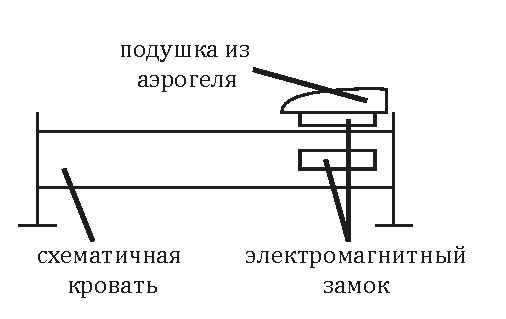
\includegraphics[width=\textwidth]{magnet_alarm_bed}
    \caption{Магнитный будильник. Версия \( 1.054571800(13) \)}
\end{figure}

\begin{itemize}
    \item Приложение для телефона. Составлять 2-, 4-стишья на иностранном языке из имеющегося набора слов для улучшения обучения.
    \begin{flushleft}
        \begin{verse}
        If you get in a pub\\
        And you have a sullen face ---\\
        Then don't stand up\\
        From out your place!
        \end{verse}

        \begin{verse}
        Do you walk to a park?\\
        Go round a place of dark!
        \end{verse}
    \end{flushleft}
    \item Острые безопасные ножи для общепита.

    \item (в помощь платной медицине) Разработка терминов для новых типов заболеваний:
        \begin{itemize}
            \item имуноизбыток
            \item сфокусированный склероз
            \item нетипичная депрессия
            \item синфазия, $\pi$-фазия, $2\pi$-фазия, ...
            \item алкофобия
            \item униполярное растройство личности
            \item соница (студенческое заболевание)
            \item неэффективное растройство
            \item торсионный шок
        \end{itemize}
    \item Cоставлять микротесты в стиле продолжите слово "сме..."
    \begin{itemize}
        \item[] ..рть/рч - у вас депрессия
        \item[] ..х - вы любите математику
        \item[] ..калка - вы не пропадёте по жизни
        \item[] ..ркалось - бросайте смотреть Задорнова
        \item[] ..тана - не хлебом единым, товарищи!
    \end{itemize}
    \item Курсы по избавлению от тавтологической зависимости "Язык язычника": расширяем ваши словестные горизонты и синонимично обогощаем вашу речь.
    \begin{figure}[ht!]
        \centering
        
\includegraphics[width=\textwidth]{taf}
    \end{figure}
    \item Приложение для иностранцев в помощь изучения великого и (все?-) могущего: составление осмысленных предложений со словами противоположного толка.
        \begin{itemize}
            \item чистый прикладник
            \item света нагорело тьма
            \item звенящая тишина
            \item обжигающий мороз
            \item сыт по горло голодовкой
        \end{itemize}
    \item Придумать устройство, которое будет проверять пространственно-временную уникальность идеи.
    \item Создать обьективную комиссию для оценки реальной стоимости субьективных вещей: произведений искусства, кино, музыки, идей и т.д.
    \item Снимать фильмы, помогающие проводить проверку психического состояния человека.
    Кличко. Игра в имитацию (смысла) \\
    Анонс:\\
    \emph{Смотреть во всех кинотеатрах, чтобы увидеть, могут все, но не все из многих могут в кинотеатрах, а, точнее, никто из никого не посмотрит, но точно не смогут смочь, кроме тех, кто увидел посмотря.}
    \item Гоблинизатор --- научные статьи словами гоблина.
    \item Делать рекламу товара так, что он будет выглядеть как наркотик.

    \begin{figure}[ht!]
        \centering
        
\includegraphics[width=\textwidth]{drug}
        \caption{Покупайте новый чай Lip Ton. Теперь ромашковый!}
    \end{figure}
    
    \item Неоархеология --- археология современности.
    
    % завершающий стартап
    \emph{От молодых специалистов требуется опыт работы, поэтому возникает следующая идея:}
    \item Организовать фирму, которая бы предоставляла опыт работы ещё на этапе студенчества. Извлечение прибыли для такой фирмы: использование набранного персонала в качестве игроков в онлайн-играх (покер и другие коммертизированные). Другой способ заработка --- различные вариации мелкого мошенничества. но это уже история совсем другого стартапа... 
\end{itemize}
